\documentclass[11pt]{report}
\usepackage[utf8]{inputenc}
\usepackage{graphicx}
\usepackage[margin=1.2in]{geometry}
\usepackage{listings}
\usepackage{fancyhdr}

\usepackage[english]{babel}
\setlength{\parindent}{4em}
\setlength{\parskip}{1em}
\renewcommand{\baselinestretch}{1.5}

\graphicspath{ {images/} }

 
\pagestyle{fancy}
\fancyhf{}
\lhead{}
\chead{}
\rhead{\textit{AURO}}
\lfoot{\textit{Dept. of CSE, VJCET}}
\renewcommand{\headrulewidth}{0pt}

\begin{document}

\begin{titlepage}
    \begin{center}
        
\Huge
        \textbf{AURO}
        
        \vspace{1cm}
        \large \textbf{MINI PROJECT REPORT}
        
        \vspace{.4cm}
		\textit{Submitted By}
		
		\vspace{.4cm}      
        \large \textbf{GINU MATHEW \hspace{.5cm} 14019917}\\
        
        \vspace{.6cm}
        \textit{In partial fulfillment for the award of degree of} \\
        
        \vspace{.4cm}
        \large \textbf{Bachelor of Technology}\\
        \vspace{.4cm}
        in \\
        \vspace{.4cm}
        \large \textbf{Computer Science \& Engineering} \\
        \vspace{0.1cm}
		\large \textbf{Mahatma Gandhi University, Kottayam}
        
        \vspace{0.4cm}
        
        
\includegraphics{vjcet.jpg}
                
        \vspace{0.4cm}
        
        \normalsize \textbf {DEPARTMENT OF COMPUTER SCIENCE \& ENGINEERING}\\
        \vspace{.4cm}
        \large \textbf {VISWAJYOTHI COLLEGE OF ENGINEERING \& TECHNOLOGY, VAZHAKULAM}
        
    \end{center}
\end{titlepage}

\begin{titlepage}
    \begin{center}
        
        \Huge
        \textbf{AURO}
        
        \vspace{1cm}
        \large \textbf{MINI PROJECT REPORT}
        
        \vspace{.4cm}
		\textit{Submitted By}
		
		\vspace{.4cm}      
        \large \textbf{GINU MATHEW \hspace{.5cm} 14019917}\\
        
        \vspace{.6cm}
        \textit{In partial fulfillment for the award of degree of} \\
        
        \vspace{.4cm}
        \large \textbf{Bachelor of Technology}\\
        \vspace{.4cm}
        in \\
        \vspace{.4cm}
        \large \textbf{Computer Science \& Engineering} \\
        \vspace{0.1cm}
		\large \textbf{Mahatma Gandhi University, Kottayam}
        
		\vspace{0.4cm}
		\textit{Under the guidance of}
		
		\vspace{0.4cm}
		\large\textbf{Mrs. RITTY JACOB\\ Assistant Professor, Department of CSE}       
        
        \vspace{0.4cm}
        
        
\includegraphics{vjcet.jpg}
        
        \vspace{0.4cm}
        
        \normalsize \textbf {DEPARTMENT OF COMPUTER SCIENCE \& ENGINEERING}\\
        \vspace{.4cm}
        \large \textbf {VISWAJYOTHI COLLEGE OF ENGINEERING \& TECHNOLOGY, VAZHAKULAM}
        
        \vspace{0.4cm}
        \normalsize \textbf{April 2017}
        
    \end{center}
\end{titlepage}

\newpage
\thispagestyle{empty}
\begin{center}
\large \textbf {VISWAJYOTHI COLLEGE OF ENGINEERING \& TECHNOLOGY, VAZHAKULAM}\\
\vspace{.4cm}
\normalsize \textbf{Department of Computer Science and Engineering}
\vspace{.6cm}

\normalsize \textbf{Mission}
\end{center}
\begin{enumerate}

\item Foster the principles and practices of computer science to empower life-long learning and build careers in software and hardware development.

\item Impart value education to elevate students to be successful, ethical and effective problem-solvers to serve the needs of the industry, government, society and the scientific community.
 
\item Promote industry interaction to pursue new technologies in Computer Science and provide excellent infrastructure to engage faculty and students in scholarly research activities.
\end{enumerate}

\begin{center}
Program Educational Objectives
\end{center}
Our Graduates 

\begin{enumerate}
1. Shall have creative and critical reasoning skills to solve technical problems ethically and responsibly to serve the society.
2. Shall have competency to collaborate as a team member and team leader to address social, technical and engineering challenges.
3. Shall have ability to contribute to the development of the next generation of information technology either through innovative research or through practice in a corporate setting.
4. Shall have potential to build start-up companies with the foundations, knowledge and experience they acquired from undergraduate education.
\end{enumerate}

\begin{center}
Program Outcomes
\end{center}

\begin{enumerate}
\item Engineering knowledge: Apply the knowledge of mathematics, science, engineering fundamentals, and an engineering specialization to the solution of complex engineering problems. 
\item Problem analysis: Identify, formulate, review research literature, and analyze complex engineering problems reaching substantiated conclusions using first principles of mathematics, natural sciences, and engineering sciences. 
\item Design / development of solutions: Design solutions for complex engineering problems and design system components or processes that meet the specified needs with appropriate consideration for the public health and safety, and the cultural, societal, and environmental considerations. 
\item Conduct investigations of complex problems: Use research-based knowledge and research methods including design of experiments, analysis and interpretation of data, and synthesis of the information to provide valid conclusions. 
\item Modern tool usage: Create, select, and apply appropriate techniques, resources, and modern engineering and IT tools including prediction and modeling to complex engineering activities with an understanding of the limitations. 
\item The engineer and society: Apply reasoning informed by the contextual knowledge to assess societal, health, safety, legal and cultural issues and the consequent responsibilities relevant to the professional engineering practice. 
\item Environment and sustainability: Understand the impact of the professional engineering solutions in societal and environmental contexts, and demonstrate the knowledge of, and need for sustainable development. 
\item Ethics: Apply ethical principles and commit to professional ethics and responsibilities and norms of the engineering practice.
\item Individual and team work: Function effectively as an individual, and as a member or leader in diverse teams, and in multidisciplinary settings. 
\item Communication: Communicate effectively on complex engineering activities with the engineering community and with society at large, such as, being able to comprehend and write effective reports and design documentation, make effective presentations, and give and receive clear instructions. 
\item Project management and finance: Demonstrate knowledge and understanding of the engineering and management principles and apply these to one’s own work, as a member and leader in a team, to manage projects and in multidisciplinary environments. 
\item Life-long learning: Recognize the need for, and have the preparation and ability to engage in independent and life-long learning in the broadest context of technological change.
\end{enumerate}

\begin{center}
Program Specific Outcomes
\end{center}

\begin{enumerate}
\item Ability to integrate theory and practice to construct software systems of varying complexity.
\item Able to Apply Computer Science skills, tools and mathematical techniques to analyze, design and model complex systems.
\item Ability to design and manage small-scale projects to develop a career in a related industry.
\end{enumerate}


\newpage
\thispagestyle{empty}
\begin{center}
\large \textbf{DECLARATION BY THE CANDIDATE}
\end{center}
\vspace{1cm}
I hereby declare that the mini-project report entitled \textbf{``AURO"} submitted by me to the Department of Computer Science \& Engineering, Viswajyothi College of Engineering \& Technology, Vazhakulam in partial fulfillment of the requirement for the award of the degree of \textbf{Bachelor of Technology} in \textbf{Computer Science \& Engineering} is a record of bonafide project work carried out by us under the guidance of \textbf{Mrs. Ritty Jacob}. I futher declare that the work reported in this project has not been submitted, either in part or in full, for the award of any other degree in this college.

\vspace{3cm}
\begin{flushright}
\textbf{Ginu Mathew}
\end{flushright}

\newpage
\thispagestyle{empty}
    \begin{center}
        
        \large
        \textbf{VISWAJYOTHI COLLEGE OF ENGINEERING \& TECHNOLOGY, VAZHAKULAM}
        
        \vspace{.4cm}
        \large \textbf{Department of Computer Science \& Engineering }
        
		\vspace{0.4cm}        
        
        
\includegraphics{vjcet.jpg}
        
        \vspace{0.8cm}
        
        \large \textbf{BONAFIDE CERTIFICATE}
        \vspace{0.4cm}
    \end{center}
This is to certify that the Mini Project report entitled \textbf{``AURO"} is a bonafide record of the work by \textbf{GINU MATHEW (14019917)} in partial fulfillment of the requirements for the award of the degree of \textbf{Bachelor of Technology} in \textbf{Computer Science \& Engineering} of Mahatma Gandhi University, Kottayam.
\\
\begin{tabular}[t]{@{}l}
Date:\\
Place: Vazhakulam\\
\rule{1cm}{0cm}\\ \\ \\
\textbf{Mrs. Nimmy George} \\
\textbf{Mini Project Coordinator}
\rule{1cm}{0cm}\\ \\ \\ \\ \\ \\ \\
\textbf{Internal Examiner}
\end{tabular}
\hfill
\begin{tabular}[t]{l@{}}
\textbf{Mrs. Ritty Jacob} \\
\textbf{Mini Project Guide}\\
\rule{1cm}{0cm}\\ \\ \\
\textbf{Dr. K.N Ramachandran Nair} \\
\textbf{Professor and HOD}\\

\rule{1cm}{0cm}\\ \\ \\ \\ \\ \\
\textbf{Internal Examiner}
\end{tabular}


\newpage
\thispagestyle{empty}
\begin{center}
\Large \textbf{ACKNOWLEDGEMENT}
\vspace{1cm}
\end{center}
First and foremost I thank God Almighty for His divine grace and blessings in making this project possible. May he continue to lead me in the years to come. It is my privilege to render heartfelt thanks and gratitude to our most beloved Manager, \textbf{Msgr. George Oliapuram} and Principal, \textbf{Dr. JosephKunju Paul C.} for providing the opportunity to do this project during the third year (2017) of our B.Tech degree course. I am deeply thankful to the Head of the Department, \textbf{Dr. K.N Ramachandran Nair} for his support and encouragement. I would like to express my sincere gratitude to my project guide \newline \textbf{ Mrs. Ritty Jacob}, Asst. Professor, Department of Computer Science and Engineering for her motivation, assistance and help for the project. I also express sincere thanks to the project coordinator \textbf{Mrs. Nimmy George}, Asst. Professor, Department of Computer Science and Engineering for her guidance and support. I also thank all the staff members of the Computer Science Department for providing their assistance and support. Last, but not the least I thank all my friends and family for their valuable feedback from time to time as well as their help and encouragement. I hereby apologize for any kind of omissions that may have taken place by mistake.

\vspace{3cm}
\begin{flushright}
\textbf{Ginu Mathew}
\end{flushright}

\newpage
\thispagestyle{empty}
\begin{center}
\Large \textbf{ABSTRACT}
\vspace{1cm}
\end{center}
Our common understanding of a personal assistant is that of a person (or an agent) who is able to provide distinct help at a given time and in a given activity context. We must be very much familiar with the commercial products such as Apple’s Siri, Google’s Now and api.ai’s Speak to It Assistant which are the necessary technology inventions (ie., composition of Natural Language Processing, Auto Speech synthesis, Dialogue management and Text-speech Processing) during the past 5 years. The possible application scenario have progressively been changing and now involves domains such as healthCare, weather forecast, navigation, translation, information and tutoring. This personal assistant (AURO) can be used to respond to simple questions and arithmetic calculations.

\tableofcontents
\thispagestyle{empty}

\listoffigures
\thispagestyle{empty}

\newpage
\thispagestyle{empty}
\begin{center}

\Large \textbf{LIST OF ABBREVIATIONS}

\vspace{1cm}

\begin{tabular}{l l}
SRS & Software Requirements Specification \\
DFD & Data Flow Diagram
\end{tabular}
\end{center}

\clearpage
\pagestyle{palin}
\setcounter{page}{1}
\chapter{PREAMBLE}

\section{Problem defenition}
In the current system, required answers to the questions are obtained by accessing web browsers and searching several websites which is time - consuming. The proposed system Auro is a solution to this problem which provide the answers in just a single step and thereby reducing the wastage of time.
\section{Objective}
The main objective of our proposed project is to build a simple personal assistant which is able to accept commands in the form of text (natural language: English) and respond back again in text (natural language). This project is implemented by Machine Learning (ML) and Natural Language Processing (NLP).  

\section{Scope}
The scope of this product is to provide an efficient and enhanced tool for the users to perform various operations quickly and more efficiently.  It finds application in many fields such as medical, educational etc.  This project is actually a demonstration of Machine learning and Natural Language Processing.  The main objective of the proposed system is to convert machines to user friendly devices through the use the use of Machine Learning and Natural Language processing.

\section{Introduction to the project}
We would have wished to use a single program just to get the answers in one go.  But what we do nowadays is that we have to scroll through different applications or different websites and search hard to get what we actually want.  The proposed system is a solution to this problem.  The project is to build a Personal Digital Assistant which is able to accept queries in the form of text (English) and respond back accordingly.  This application can be used to get or fetch the user required processes based on the input provided.  This document is intended for both the stakeholders and the developers of the software and will be proposed to the committee for its approval.

\chapter{SYSTEM STUDY}
\section{Introduction}
\subsection*{Purpose}
Nowadays we have to scroll and search hard and need to go through different applications to get what we actually want.  Our proposed system is a solution to this problem.  The project is to build a personal digital assistant which is able to accept queries in the form of text (English) and respond back.  This application can be used to get or fetch the user required process based on the input provided.  This document is intended for both the stakeholders and the developers of the software and will be proposed to the committee for its approval.

\subsection*{Document Conventions}
All system development activities should follow the final version of this document.  Any discrepancy that found during in later phases should be modified subject to SRS.  However, this document may be subjected to change depending on the decision of the group members.
\newline
The typographical conventions used in writing this SRS are:
\begin{itemize}
\item SRS main headings : font = Times New Roman, Bold, size = 18
\item SRS sub headings  : font = Times New Roman, Bold, size=14
\item SRS Body text     : font = Times New Roman, size = 12
\end{itemize}
Header and footer font size =10,  Italics, Times New Roman.  The document contains header and footer on all pages.  Header is the name of the project on the top-left end and page number.
Bullets are used to denote main points in the section.
\subsection*{Intended Audience and Reading Suggestion}
This document contains general information based on our Mini Project on building a personal digital assistant which will be implemented using python programming language.
The document is intended for different types of users such as:
\newline
\textbf{Administrators}:  In order to be sure they are developing the right project that fulfills
requirements provided in this document.
\newline
\textbf{Developers}: In order to be sure they are developing the right project that fulfills
requirements provided in this document.
\newline
\textbf{Testers}: In order to have an exact list of features and functions that have to respond according to requirements and provided diagrams. 
\newline
\textbf{Users}:​ ​ In order to get familiar with the idea of the project and suggest other features that would make it even more functional.
\newline
The topics are in their increasing order of specificity. The rest of the SRS contain overall description, external interface requirements, system features and other non-functional requirements.                               
\subsection*{Product Scope}
The scope of this product is to provide an efficient and enhanced tool for the users to perform various operations quickly and more efficiently.  It finds application in many fields such as medical, educational etc.  Our project is actually a demonstration of Machine learning and Natural Language Processing.  The main objective of the proposed system is to convert machines to user friendly devices through the use the use of Machine Learning and Natural Language processing. 

\section{Overall Description}
\subsection*{Product Perspective}
In this project, we present an implementation of a Personal Digital Assistant - AURO, which is  able to understand the inputs given to the computer (in English) by the user, analyze the sentence and produce the desired output.
\subsection*{User Classes and Characteristics}
We have only one user class since we don’t have any security levels or privilege levels.  Our user base includes any user who uses AURO app.  The users of this project is global i.e., anyone can be the user of this application.  This application is meant to be used based on the application the project is implemented.  Our project is made as a demonstration of Natural Language Processing and Artificial Intelligence. 
\section{External Interface Requirements}
\subsection*{User Interfaces}
The user interface for this project is through a web browser.  A chat box is provided so that the user is able to enter his query or sentence as input.
\subsection*{Hardware Interfaces}
The entire software require completely equipped computer system including monitor, keyboard and mouse.
\subsection*{Software Interfaces}
The system uses Natural Language ToolKit (NLTK), a python package for natural language processing.  NLTK requires python 2.7 or above versions. 
\subsection*{Communication Interfaces}
The system requires an active internet in order to access the data from the data store.  
\section{System Features}
\textbf{AURO} is an application that accepts commands from the user in the form of text (natural language) and reply back again in text (natural language).
\subsection*{Tokenize the inputs from the user}

\subsubsection*{Description and priority}
In lexical analysis, tokenization is the process of breaking a stream of text up into words, phrases, symbols, or other meaningful elements called tokens. The list of tokens becomes input for further processing such as parsing or text mining.  This feature is very much important as each word has to be extracted separately in order to choose and analyze the question of the user.

\subsubsection*{Functional Requirement}
FREQ-1: Any question or input provided by the user.


\subsection*{Filter appropriate Keywords from the tokenized input}
\subsubsection*{Description and Priority}
This feature analyzes the important terms or words from the tokenized user input so as to analyze the need of the user and to provide the user with the required output.

\subsection*{Form and process Querry}
\subsubsection*{Description and Priority}
This feature forms and process the query which will be compared with data in the database and give required output. 

\section{Non-functional Requirements}
\subsection*{Performance Requirements}
The performance of system lies in the way it is handled.  The other factor of performance is the absence of any suggested requirements.

\subsection*{Safety Requirements}
No such safety requirement is needed.

\subsection*{Security Requirements}
No such security requirement is needed.
\
\subsection*{Software Quality Attributes}
\begin{enumerate}
\item \textbf{Easy to operate}: The system should be easy to operate and limited to the budget of the user.
\item \textbf{Accuracy}: The accuracy of the proposed system is moderate.
\end{enumerate}

\section{System Specification}
The system specification includes basic software and hardware used for implementing or developing this project which is an important factor for the project.

\subsection{Software Specification}
The selection of an appropriate software for devolopment is an important task, since completion of the system is greatly dependent on software selected. The different software used AURO includes :
\subsubsection*{Python}
Python is an interpreted, general-purpose high-level programming language whose design philosophy emphasizes code readability. Python aims to combine "remarkable power with very clear syntax" and its standard library is large and comprehensive. Its use of indentation for block delimiters is unique among popular programming languages.\newline
Python supports multiple programming paradigms, primarily but not limited to object-oriented, imperative and, to a lesser extent, functional programming styles. It features a fully dynamic type system and automatic memory management, similar to that of Scheme, Ruby, Perl, and Tcl. Like other dynamic languages, Python is often used as a scripting language, but is also used in a wide range of non-scripting contexts. Python interpreters are available for many operating systems, and Python programs can be packaged into stand-alone executable code for many systems using various tools. Python is a multi-paradigm programming language.
\newline
Rather than forcing programmers to adopt a particular style of programming, it permits several styles: object-oriented programming and structured programming are fully supported, and there are a number of language features which support functional programming and aspect-oriented programming.
\newline
Python uses dynamic typing and a combination of reference counting and a cycle-detecting garbage collector for memory management. An important feature of Python is dynamic name resolution, which binds method and variable names during program execution.
\newline
Rather than requiring all desired functionality to be built into the language's core, Python was designed to be highly extensible. The design of Python offers only limited support for functional programming in the Lisp tradition.
\newline
Python was intended to be a highly readable language. It is designed to have an uncluttered visual layout, frequently using English keywords where other languages use punctuation. Python requires less boilerplate than traditional manifestly typed structured languages such as C or Pascal, and has a smaller number of syntactic exceptions and special cases than either of these.
\newline
Python uses whitespace indentation, rather than curly braces or keywords, to delimit blocks. An increase in indentation comes after certain statements; a decrease in indentation signifies the end of the current block.
\newline
Python uses duck typing and has typed objects but untyped variable names. Type constraints are not checked at compile time; rather, operations on an object may fail, signifying that the given object is not of a suitable type. Despite being dynamically typed, Python is strongly typed, forbidding operations that are not well-defined rather than silently attempting to make sense of them.
\newline
Python allows programmers to define their own types using classes, which are most often used for object-oriented programming. New instances of classes are constructed by calling the class, and the classes themselves are instances of the metaclass type , allowing metaprogramming and reflection.

\subsubsection*{Django}
Django is a free and open source web application framework, written in Python. A web framework is a set of components that helps you to develop websites faster and easier. When you are  building a website, you always need a similar set of components: a way to handle user authentication (signing up, signing in, signing out), a management panel for your website, forms, a way to upload files, etc. Django give us the ready made components to use. These framework help to reduce the burden of building a new site. The web server reads the letter and then sends a response with a webpage. The django is used to create the content of the webpage.
\newline
When a request comes to a web server, it is passed to Django which tries to figure out what is actually requested. It takes a web page address first and tries to figure out what to do. This part is done by Django's urlresolver. It is not very smart – it takes a list of patterns and tries to match the URL. Django checks patterns from top to bottom and if something is matched, then Django passes the request to the associated function (which is called view).

\subsubsection*{jQuery}
jQuery is a fast, small, and feature-rich JavaScript library. It makes things like HTML document traversal and manipulation, event handling, animation, and Ajax much simpler with an easy-to-use API that works across a multitude of browsers.
\newline
The purpose of jQuery is to make it much easier to use JavaScript on your website. jQuery takes a lot of common tasks that require many lines of JavaScript code to accomplish, and wraps them into methods that you can call with a single line of code.

\subsubsection*{Heroku}
Heroku is a cloud Platform-as-a-Service (PaaS) supporting several programming languages that is used as a web application deployment model.  Heroku, one of the first cloud platforms, has been in development since June 2007, when it supported only the Ruby programming language, but now supports Java, Node.js, Scala, Clojure, Python, PHP, and Go.  For this reason, Heroku is said to be a polyglot platform as it lets the developer build, run and scale applications in a similar manner across all the languages. 
\newline
Applications that are run from the Heroku server use the Heroku DNS Server to direct to the application domain (typically ``applicationname.herokuapp.com").  Each of the application containers, or dynos, are spread across a ``dyno grid" which consists of several servers.  Heroku's Git server handles application repository pushes from permitted users.

\subsubsection*{Natural Language Toolkit}
The Natural Language Toolkit (NLTK) is a Python package for natural language processing. NLTK requires Python 2.7, or 3.4+. NLTK is a leading platform for building Python programs to work with human language data. It provides easy-to-use interfaces to over 50 corpora and lexical resources such as WordNet, along with a suite of text processing libraries for classification, tokenization, stemming, tagging, parsing, and semantic reasoning, wrappers for industrial-strength NLP libraries.
\newline
NLTK is suitable for linguists, engineers, students, educators, researchers, and industry users alike. NLTK is available for Windows, Mac OS X, and Linux.

\subsubsection*{Git}
Git is a version control system(VCS) for tracking changes in computer files and coordinating work on those files among multiple people.  It is primarily used for software development, but it can be used to keep track of changes in any files.  As a distributed revision control system it is aimed at speed, data integrity, and support for distributed, non-linear workflows.
\newline
Git was created by Linus Torvalds in 2005 for development of the Linux kernel, with other kernel developers contributing to its initial development.  Its current maintainer since 2005 is Junio Hamano.
\newline
As with most other distributed version control systems, and unlike most client – server systems, every Git directory on every computer is a full-fledged repository with complete history and full version tracking abilities, independent of network access or a central server.  Like the Linux kernel, Git is free software distributed under the terms of the GNU General Public License version 2.


\chapter{SYSTEM DESIGN AND MODELLING}
\section{Design Methodologies}
System design is the process of developing specifications for a candidate system that meet the criteria established in the system analysis. Major step in the system design is the preparation of the input forms and the output reports in a form applicable to the user.
\newline
The main objective of the system design is to use the package easily by any computer operator. System design is the creative act of invention, developing new inputs, a database, offline files, method, procedures and output for processing business to meet an organization objective. System design builds information gathered during the system analysis.
\newline
In design an efficient and effective system is of great importance to consider the human factor and equipment that these will require to use. System analyst must evaluate the capabilities and limitations of the personal and corresponding factors of the equipment itself. The characteristics associated with effective system operation are reaccessibility, decision making ability, economy, flexibility, reliability and simplicity.
\newline
We have followed the waterfall model. It is the simplest process model which states that the phases are organized in linear order. One of the main advantages of the model is its simplicity. It is conceptually straight forward and divide the large task of building a software system into a series of cleanly divided phases.
\newline
Waterfall model is the most widely used process model. It is well suited for routine type of projects where the requirements are well understood. That is, if developing organization is quite familiar with the problem domain and the requirements for the software are quite clear, the water fall model works well.
\subsection*{Input design}
Input design is the process of converting the user inputs to a computer-based format. The design for handling input specifies how data are accepted for computer processing. Input design is a part of overall system design that needs careful attention and if includes specifying the means which action are taken. A system user interacting through a workstation must be able to tell the system whether to accept input ,produce a report or end processing. The collection of input data is considered to be the most extensive part of the system design. The major activities carried out are:

\begin{itemize}
\item Collection of needed data from the source.
\item Conversion of data into computer accepted.
\item Verification of converted data.
\item Checking data for accuracy.
\item To ensure that input is understood by and acceptable to the user.
\end{itemize}

\subsection*{Output design}
The output design has done so that the results of processing should be communicated to the user. Effective output design will improve the clarity and performance of outputs. Output is the main reason for developing the system and the basis on which they will evaluate the usefulness of the application.
\newline
Output design phase of the system is concerned with the convergence of information to the end user-friendly manner. The output design should be efficient, intelligible so that the system relationship with the end user is improved and they‟re by enhancing the process of decision making.
Output design objectives

\begin{itemize}
\item It provides maximum information to the user according to their needs.
\item Outputs were identified and described.
 \itemProvides convenient and predicted output to the user.
\end{itemize}
The first part of our output is the detected laser spot being circled in the cam window
\section{System Architecture}
A system architecture can comprise system components that will work together to implement the overall system. 
A system architecture is a conceptual model that defines the structure, behavior, and more views of a system. An architecture description is a formal description and representation of a system, organized in a way that 
supports reasoning about the structures and behaviors of the system.
\newline
In the system architecture of AURO, the main component is the AURO API. It is the only component which is performing all the operations.  Input is accepted from the user through the AURO window. User can input the query using any device that has internet access.
\newline
Query or the input is accepted only in English language and the answer or output will be displayed after searching for it in the databases used such as Google & Wikipedia, in the same AURO window. No more components are involved here.
\vspace{1cm}
\begin{figure}[!h]
  \hspace{.3cm}
  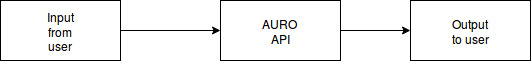
\includegraphics[width=.9\textwidth]{archt.jpg} 
  \caption{Architecture for Auro}
  \label{fig:archt}
\end{figure}

%\newpage
\section{Data Flow Diagram}
A data flow diagram (DFD) is a graphical representation of the flow of data through a system. A DFD is often used as a preliminary step to create an overview of the system without going into detail. It is used in the problem analysis. It views system as a function that atrnsforms input into the desired outputs. The data undergoes a series of transformations before it becomes the output. The data flow diagram aims to capture transformations that take place within the system to the input data so that eventually the output is produced. The agent that performs the transformation is the process. So, a DFD shows the movement of data through different processes or transformations in the system.

\subsection*{Level 0 Data Flow Diagram}
The level 0 data flow diagram shown in Figure \ref{fig:level0} contain an entity, user and the main process of the system. The user provide commands in the form of text. These commands are then converted into natural language. Further it search the database for the corresponding answer. The system retrieves the answer to user as final result.  
\begin{center}

\begin{figure}[!h]
  \hspace{2cm}
  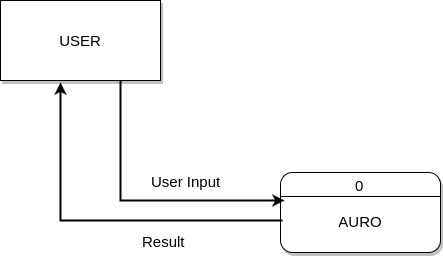
\includegraphics[width=.7\textwidth]{level0.jpg} 
  \caption{Level 0 DFD}
  \label{fig:level0}
\end{figure}
\end{center}

\subsection*{Level 1 Data Flow Diagram}
A level 1 DFD represents the system's major process, data flows and the data stores at a high level of detail.The level 1 DFD shown in Figure \ref{fig:level1} contain one external entity the user. The text command provided by the user is tokenized into words which forms group of words. From this group, the required keywords are filtered neccessary for searching the datbase. The system search database for the corresponding answer and is given to the user as the final result.
\begin{figure}[!h]
  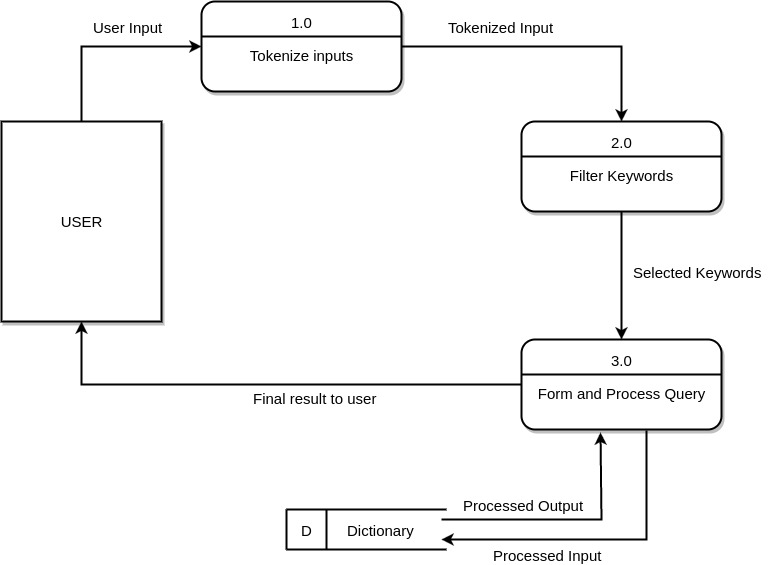
\includegraphics[width=1\textwidth]{level1.jpg}
  \caption{Level 1 DFD}
  \label{fig:level1}
\end{figure}


\newpage
\section{Use Case Diagram}
A use case diagram shown in Figure \ref{fig:usecase} is the represention  of the user's interaction with the system that shows the relationship between the user and the different use cases. The use case diagrams are also referred to as behaviour diagrams used to describe a set of actions (use cases) that some systems or should or can perform in collaboration with one or more external users of the system. Each use case should provide some observable and valuable result to the stakeholders of the system.
\newline
External entities are reffered to as actors which can be human users, external hardware or other systems. An actor is a named stick figure, or a class rectangle with $<<$actor$>>$  keyword. A use case is a single unit of meaningful work.The purpose of the use case diagrams is simply to provide the high level view of the system and convey the requirements. The use case is denoted by an ellipse.
\newline
The use case diagram of AURO consist of one external entity the user and four use cases, user input, processing the text, search datbase and display the result. The user provide input to the system which is processed into natural language by the use case processing the text.  
\begin{figure}[!h]
  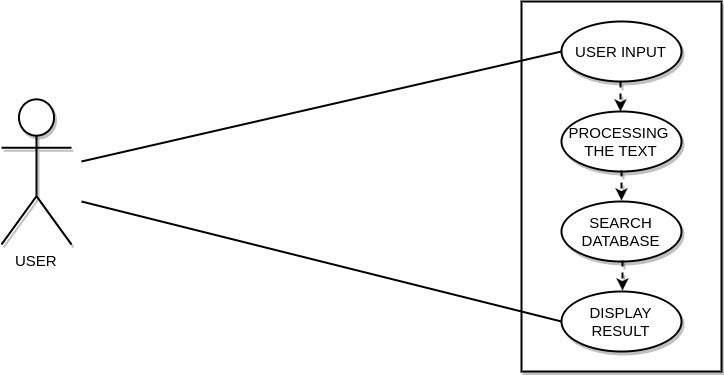
\includegraphics[width=1\textwidth]{usecase.jpg}
  \caption{Use Case Digram}
  \label{fig:usecase}
\end{figure}



\chapter{IMPLEMENTATION}
\section{Introduction}
Implementation is the stage in the project where the theoretical design is turned into a working system and is giving confidence on the new system for the users that it will work efficiently and effectively. It involves careful planning, investigation of the current system and its constraints on implementation, design of methods to achieve the change over, an evaluation, of change over methods. Apart from planning major task of preparing the implementation are education and training of users. The more complex system being implemented, the more involved will be the system analysis and the design effort required just for implementation. An implementation coordinating committee based on policies of individual organization has been appointed. The implementation process begins with preparing a plan for the implementation of the system. According to this plan, the activities are to be carried out, discussions made regarding the equipment and resources and the additional equipment has to be acquired to implement the new system.Implementation is the final and important phase. 
\newline
The most critical stage in achieving a successful new system and in giving the users confidence that the new system will work and be effective. The system can be implemented only after thorough testing is done and if it found to working according to the specification. This method also offers the greatest security since the old system can take over if the errors are found or inability to handle certain type of transactions while using the new system.

\section{Implentation Methods}
Implementation is the final and important phase. The most critical stage in achieving a successful new system and in giving the users confidence that the new system will work and be effective. The system can be implemented only after thorough testing is done and if it found to working according to the specification.
\newline
In this project, query input of our system will be tokenized word by word and from this list of tokens the NN, NNS, NNP, NNPS and CD will be identified. After filtering the keywords the necessary output will be displayed to the user.
\newline
This can be used in any field of work as it makes the searching kind of operations much more easier and faster than usual. The database can be designed specially  and specifically for our particular field of work also. This software is simple,  user-friendly and can be installed in personal computers.


\chapter{TESTING}
\section{Introduction}
Testing is the process of executing a program with the indent of finding any errors .A good test of course has the high probability of finding a yet undiscovered error. A successful testing is the one that uncovers a yet undiscovered error. A test is vital to the success of the system. System test makes a logical assumption that if all parts of the system are correct, then goal will be successfully achieved. The candidate system is subjected to a variety of tests online like responsiveness, its value, stress and security. A series of tests are performed before the system is ready for user acceptance testing. 
\newline
The success of testing in revealing errors depends on the test cases. Testing should help locate errors, not just detect their presence. Test should be organized in a way that helps isolate errors.
\newline
Thus testing should be considered only one of the means to analyze the behavior of a system and should be integrated with other verification techniques in order to enhance our confidence in system qualities as much as possible. 
\newline
System testing of software or hardware is testing conducted on a complete, integrated system to evaluate the system’s compliance with its specified requirements. System testing falls within the scope of black box testing, and as such, should require no knowledge of the inner design of the code or logic.
\newline
Black-box testing is a method of software testing that tests the functionality of an application as opposed to its internal structures or workings. Specific knowledge of the application's code/internal structure and programming knowledge in general is not required. Test cases are built around specifications and requirements, i.e., what the application is supposed to do. It uses external descriptions of the software, including specifications, requirements, and designs to derive test cases. These tests can be functional or non-functional, though usually functional. 
\newline
 The test designer selects valid and invalid inputs and determines the correct output. There is no knowledge of the test object's internal structure. This method of test can be applied to all levels of software testing: unit, integration, functional, system and acceptance. It typically comprises most if not all testing at higher levels, but can also dominate unit testing as well.  
 
\subsection*{Unit Testing}
In unit testing different modules are tested against the specification produced during the design of modules. Unit testing is essential for verification during coding phase. The aim is to test the internal logic of the modules. The tests carried out during the programming stage itself. 
\newline
This enables the tester to detect errors in coding and logic that are contained within that module alone. Those resulting from the interaction between modules are initially avoided. Unit test comprises the set of performed prior to integration of the unit in to the entire project. Four categories of tests are performed on each unit.
\newline
\textbf{Functional test}:  The code is exercised with normal input values for which the expected results are shown, as well as boundary values and values on and just outside the functional boundaries and special values such as logically related inputs. 
\newline
\textbf{Performance Test}:  Performance test is done to determine the amount of execution time spent in various parts of the unit, program throughput and response time and device utilization by the program unit. 
\newline
\textbf{Stress Test}: Stress test intentionally breaks the unit. This helps in learning about the strength and limitations of the program by examining the manner in which a program unit breaks. 
\newline
\textbf{Structure Test}: Structure tests are used to test the internal logic of a program. The major activity involved in this is to decide which paths to exercise, deriving test to exercise those paths, determining the test coverage criteria to be used. 

\subsection*{Integration Testing}
Integration testing focuses on the design and the construction of the software architecture. The data can be lost across the interface or one module can pose an adverse effect on another. The sub functions when combined may not produce the major function. Integration testing is a systematic technique for the program structure, while at the same conducting test to uncover errors associated with the interface. In this test, groups of the program modules are tested together to determine if they interface properly. Two types of integration testing are:
\newline
\textbf{Top down Integration}: This method is an incremental approach to one construction of program structure. Modules are integrated by moving downward through the control hierarchy, beginning with the main program module. The modules subordinates to the main program module are incorporated into the structure in either a depth first or breadth first manner.
\newline
\textbf{Bottom up Integration}: This method begins the construction and testing with the modules at the lowest level in the program structure. Since the modules are integrated from the bottom up, processing required for modules subordinate to a given level is always available and the need for the stubs is eliminated.

\subsection*{System Testing}
System testing is a critical element of quality assurance and represents the ultimate review of analysis, design and coding. When a system is developed it is hoped that it performs, manual procedures, computer operations and control.
\newline
System testing is the process of checking whether the developed system is working according to the objective and requirement. All testing accordance to the test conditions specified earlier. This will ensure that the test coverage meets the requirements and that testing is done in a systematic manner. 

\section{Test Cases}
A test case in software engineering is a set of conditions or variables under which a tester will determine whether an application or software system is working correctly or not. It is the mechanism for determining 
whether a software program or system has passed or failed such a test is known as a test oracle. In some
settings, an oracle could be a requirement or use case, while in others it could be a heuristics. It may take many test cases to determine that a software program or system is functioning correctly. Test cases are often referred to as test scripts, particularly when written. Written test cases are usually collected into test suites.
\vspace{2cm}
\begin{table}[h]
\begin{center}
 \begin{tabular}{ |c|c|c|c|c| } 
 \hline
 \textbf{Sno} & \textbf{Unit to test} & \textbf{Test Data} & \textbf{Expected Result} & \textbf{Status} \\  
 \hline
  1 &\begin{tabular}{@{}c@{}} Who is the president\\ of india \end{tabular} & Pranab Mukherji & Pranab Mukherji & Pass \\ 
 \hline
 2 & \begin{tabular}{@{}c@{}}What is the capital \\ of kerala \end{tabular} & Thiruvananthapuram & Thiruvananthapuram & Pass \\
 \hline
 3 & Who killed indira gandhi &  assassination | firearm  & \begin{tabular}{@{}c@{}}Satwant Singh \\ \& Beant Singh \end{tabular} & Fail \\ 
 \hline
 4 & What is president of india & Pranab Mukherji & Null & Fail \\
 \hline
 
\end{tabular}
\label{Tab 1:}
\caption{Test Case Table}
\end{center}
\end{table}

\chapter{CONCLUSION}
\section{Advantages and Disadvantages of Auro}
\subsection*{Advantages}
The main advantage of our project is that we have developed a personal assistant for the users.

\begin{enumerate}

\item We can make use of this project in many areas of work such as educational field, medical field.
\item We could make our searching operations more faster and easier.
\item This project gives us a simpler & user- friendly system that acts as a question-answering system

\end{enumerate}

\subsection*{Disadvantages}
The main disadvantage of our project is that we have developed a personal assistant that can accept text in English language only.
Some of the other disadvantages are listed below:
\begin{enumerate}

\item It can only accept text inputs and not voice or gestures as inputs.

\item Proper checking should be done to ensure that the queries are answered in a right way or else it can be a inconvenience to the user.

\item Proper internet connection is required for efficient operation of the system.

\item Auro is not fully trained to respond to 100\% correct answer.

\end{enumerate}

\section{Future Scope}
Some of the main future scope is that this project can be further extended to one which can accept voice and gestures as inputs along with text in another languages as well. In this way this project can become a good help for the users especially the disabled ones and people who are not familiar with English language.

Also this project can be again extended to level in which we can upload images through the user interface window and image searches can be done which can help users in an advanced way. One of future enhancement refers to the modification or improvements to the currently developed system. System enhancement may be required if there is change in organizational requirements of the user priorities. To carry out these changes the system have to be revaluated,programs need to be modified and then again tested for user acceptance.Future developements can be easily integrated to the system.

\newpage
\section*{APPENDIX A}

\subsection*{Main.js}
\begin{verbatim}
(function() {  
    var Message;  
    Message = function(arg) {
        this.text = arg.text, this.message_side = arg.message_side;   
        this.draw = function(_this) {   
            return function() {
                var $message;
                $message = $($('.message_template').clone().html();
                $message.addClass(_this.message_side).find('.text').html(_this.text);
                $('.messages').append($message);
                return setTimeout(function() {
                    return $message.addClass('appeared');
                }, 0);
            };
        }(this);
        return this;
    };
    $(function() {
        var lastSend;
        var getMessageText, message_side;
        message_side = 'right';
        getMessageText = function() {
            var $message_input;
            $message_input = $('.message_input');
            return $message_input.val();
        };
        sendMessage = function(text) {
            var $messages, message;
            if (text.trim() === '') {
                return;
            }
            $('.message_input').val('');
            $messages = $('.messages');
            message_side = message_side === 'left' ? 'left' : 'left';
            message = new Message({
                text: text,
                message_side: message_side
            });
            message.draw();
            return $messages.animate({
                scrollTop: $messages.prop('scrollHeight')
            }, 300);
        };
        receiveMessage = function(text) {
            var $messages, message;
            if (text.trim() === '') {
                return;
            }
            $('.message_input').val('');
            $messages = $('.messages');
            message_side = message_side === 'right' ? 'right' : 'right';
            message = new Message({
                text: text,
                message_side: message_side
            });
            message.draw();
            return $messages.animate({
                scrollTop: $messages.prop('scrollHeight')
            }, 300);
        };
        // $('.send_message').click(function(e) {
        //     lastSend = $('.message_input').val();
        //     return receiveMessage(getMessageText());
        // });
        $('.message_input').keyup(function(e) {
            lastSend = $('.message_input').val();
            if (e.which === 13) {
                 var user_data=lastSend;
                console.log(user_data);
                RequestAPI(user_data);
                return receiveMessage(getMessageText());
            }
        });
        sendMessage('Hello User! What would you like to know?');
        $('#send_button').on('click',function(){
            var user_data=lastSend;
            console.log(user_data);
            RequestAPI(user_data);
        });
    });
}.call(this))
function RequestAPI(request_data){
    myURL = 'https://auro-api.herokuapp.com/api/?q=' + request_data;
        var api_reply;
        var ourRequest = new XMLHttpRequest();
        ourRequest.open('GET', myURL);
        ourRequest.onreadystatechange=function(){
            if(this.readyState==4 && this.status==200){
                api_reply=this.responseText;
                // console.log(api_reply);
                sendMessage(api_reply);
            }
        }
        ourRequest.open('GET', myURL, true);
        ourRequest.send();
}
\end{verbatim}
\newpage
\subsection*{Code for User Interface Window}
\begin{verbatim}
<!DOCTYPE html>
<html>

<head>
    <title>AURO</title>
    <meta charset="utf-8">
    <meta name="viewport" content="width=device-width, initial-scale=1">
    
    <link rel="stylesheet"
     href="https://maxcdn.bootstrapcdn.com/bootstrap/3.3.7/css/bootstrap.min.css">

    <script src="https://code.jquery.com/jquery-3.2.1.min.js" 
    		integrity="sha256-hwg4gsxgFZhOsEEamdOYGBf13FyQuiTwlAQgxVSNgt4=" 
    		crossorigin="anonymous">
    	</script>

    <link 
    href="https://maxcdn.bootstrapcdn.com/bootstrap/3.3.7/css/bootstrap.min.css">

    <script src="https://maxcdn.bootstrapcdn.com/bootstrap/3.3.7/js/bootstrap.min.js">
    </script>

    <link rel="shortcut icon" type="image/x-icon "href="./res/logo.png" />

    <style type="text/css">
        * {
            box-sizing: border-box;
        }
        body {
            background-color: #edeff2;
            font-family: "Calibri", "Roboto", sans-serif;
        }
        .navbar {
            padding-top: 7px;
            padding-bottom: 7px;
            border: 0;
            border-radius: 0;
            margin-bottom: 0;
            font-size: 16spx;
            letter-spacing: 5px;
        }
        .navbar-nav  li a:hover {
            color: #1abc9c !important;
        }
        .chat_window {
            position: absolute;
            width: calc(100% - 20px);
            max-width: 800px;
            height: 500px;
            border-radius: 10px;
            background-color: #fff;
            left: 50%;
            top: 50%;
            transform: translateX(-50%) translateY(-50%);
            box-shadow: 0 10px 20px rgba(0, 0, 0, 0.15);
            background-color: #f8f8f8;
            overflow: hidden;
        }
        
        .top_menu {
            background-color: #fff;
            width: 100%;
            padding: 20px 0 15px;
            box-shadow: 0 1px 30px rgba(0, 0, 0, 0.1);
        }
        
        .top_menu .buttons {
            margin: 3px 0 0 20px;
            position: absolute;
        }
        
        .top_menu .buttons .button {
            width: 16px;
            height: 16px;
            border-radius: 50%;
            display: inline-block;
            margin-right: 10px;
            position: relative;
        }
        
        .top_menu .buttons .button.close {
            background-color: #f5886e;
        }
        
        .top_menu .buttons .button.minimize {
            background-color: #fdbf68;
        }
        
        .top_menu .buttons .button.maximize {
            background-color: #a3d063;
        }
        
        .top_menu .title {
            text-align: center;
            color: #bcbdc0;
            font-size: 20px;
        }
        
        .messages {
            position: relative;
            list-style: none;
            padding: 20px 10px 0 10px;
            margin: 0;
            height: 347px;
            overflow: scroll;
        }
        
        .messages .message {
            clear: both;
            overflow: hidden;
            margin-bottom: 20px;
            transition: all 0.5s linear;
            opacity: 0;
        }
        
        .messages .message.left .avatar {
            background-color: #f5886e;
            float: left;
        }
        
        .messages .message.left .text_wrapper {
            background-color: #ffe6cb;
            margin-left: 20px;
        }
        
        .messages .message.left .text_wrapper::after,
        .messages .message.left .text_wrapper::before {
            right: 100%;
            border-right-color: #ffe6cb;
        }
        
        .messages .message.left .text {
            color: #c48843;
        }
        
        .messages .message.right .avatar {
            background-color: #fdbf68;
            float: right;
        }
        
        .messages .message.right .text_wrapper {
            background-color: #c7eafc;
            margin-right: 20px;
            float: right;
        }
        
        .messages .message.right .text_wrapper::after,
        .messages .message.right .text_wrapper::before {
            left: 100%;
            border-left-color: #c7eafc;
        }
        
        .messages .message.right .text {
            color: #45829b;
        }
        
        .messages .message.appeared {
            opacity: 1;
        }
        
        .messages .message .avatar {
            width: 60px;
            height: 60px;
            border-radius: 50%;
            display: inline-block;
        }
        
        .messages .message .text_wrapper {
            display: inline-block;
            padding: 20px;
            border-radius: 6px;
            width: calc(100% - 85px);
            min-width: 100px;
            position: relative;
        }
        
        .messages .message .text_wrapper::after,
        .messages .message .text_wrapper:before {
            top: 18px;
            border: solid transparent;
            content: " ";
            height: 0;
            width: 0;
            position: absolute;
            pointer-events: none;
        }
        
        .messages .message .text_wrapper::after {
            border-width: 13px;
            margin-top: 0px;
        }
        
        .messages .message .text_wrapper::before {
            border-width: 15px;
            margin-top: -2px;
        }
        
        .messages .message .text_wrapper .text {
            font-size: 18px;
            font-weight: 300;
        }
        
        .bottom_wrapper {
            position: relative;
            width: 100%;
            background-color: #fff;
            padding: 20px 20px;
            position: absolute;
            bottom: 0;
        }
        
        .bottom_wrapper .message_input_wrapper {
            display: inline-block;
            height: 50px;
            border-radius: 25px;
            border: 1px solid #bcbdc0;
            width: calc(100% - 160px);
            position: relative;
            padding: 0 20px;
        }
        
        .bottom_wrapper .message_input_wrapper .message_input {
            border: none;
            height: 100%;
            box-sizing: border-box;
            width: calc(100% - 40px);
            position: absolute;
            outline-width: 0;
            color: gray;
        }
        
        .bottom_wrapper .send_message {
            width: 140px;
            height: 50px;
            display: inline-block;
            border-radius: 50px;
            background-color: #a3d063;
            border: 2px solid #a3d063;
            color: #fff;
            cursor: pointer;
            transition: all 0.2s linear;
            text-align: center;
            float: right;
        }
        
        .bottom_wrapper .send_message:hover {
            color: #a3d063;
            background-color: #fff;
        }
        
        .bottom_wrapper .send_message .text {
            font-size: 18px;
            font-weight: 300;
            display: inline-block;
            line-height: 48px;
        }
        
        .message_template {
            display: none;
        }
        .container-fluid {
            padding-top: 5px;
            padding-bottom: 5px;
        }
    </style>

</head>

<body>

    <nav class="navbar navbar-default">
        <div class="container">
            <div class="navbar-header">
                <a class="navbar-brand avatar" href="#">
                <img src="./res/img1.png" class = "img-circle" width="90px" height="90px"></a>
            </div>
            
        </div>
    </nav>
    <div class="chat_window">
        <div class="top_menu">
            <div class="title">AURO - The Personal Digital Assistant</div>
        </div>
        <ul class="messages"></ul>
        <div class="bottom_wrapper clearfix">
            <div class="message_input_wrapper">
              <input class="message_input" placeholder="Type your message here..." 
              id="user_input"/>
            </div>
            <div class="send_message" id="send_button">
                <div class="icon"></div>
                <div class="text">Send</div>
            </div>
        </div>
    </div>
    <div class="message_template">
        <li class="message">
            <div class="avatar" ><img src="./res/assistant.png" 
            class="img-circle" width="60px" height="60px"></div>
            <div class="text_wrapper">
                <div class="text"><p id="reply"></p></div>
            </div>
        </li>
    </div>
    

    <footer class="container-fluid text-center">
        <p align="center">A MiniProject by 
			<a href="https://www.github.com/SooluThomas" target="_blank">Soolu</a>, 
			<a href="https://github.com/ginu123" target="_blank">Ginu</a> and 
			<a href="https://www.facebook.com/greeshma.mathew.79"
				 target="_blank">Greeshma</a>
		</p> 
    </footer>

    <script src = "./js/main.js"></script>
</body>

</html>
\end{verbatim}
\newpage

\section*{Code for API}

\begin{lstlisting}
# -*- coding: utf-8 -*-
from __future__ import unicode_literals

from django.shortcuts import render
from django.http import HttpResponse

import wikipedia
import wolframalpha

from nltk.tokenize import PunktSentenceTokenizer
import nltk

from tensorflow.examples.tutorials.mnist import input_data
mnist = input_data.read_data_sets("MNIST_data/", one_hot=True)
import tensorflow as tf

def tokenStr():
	filename = "./Files/userinput.txt"
	filename1 = "./Files/dictionary.txt"
	user = input("Enter Data: ")

	with open (filename, "w") as fd:
		fd.write(user)

	fd = open(filename,"r")
	print(fd.read())
	fd.close()

	fd = open(filename, "r")
	fd1 = open(filename1, "r")
	train_text = fd.read()
	# sample_tect = fd1.read()


	custom_sent_tokenizer = PunktSentenceTokenizer(train_text)

	tokenized = custom_sent_tokenizer.tokenize(train_text)

	def process_content():
		try:
			for i in tokenized[:5]:
				words = nltk.word_tokenize(i)
				tagged = nltk.pos_tag(words)
				print(tagged)
				with open("./Files/tokenized.txt", "w") as fd, 
				open(filename) as fd1, open("./Files/comp.txt") as fd2:
					# myWords = set(line.split(',') for line in tagged)
					with open("./Files/newtokens.txt", "w") as f:
						for line in tagged:
							print(line)
							freq1 = line[1]
							f.write(line + "\n")
						for line1 in fd2:
							freq= line1[1]
							if freq in freq1:
								print(freq)
								# fd.write(myWords)
				fd.close()
				chunkGram = r"""Chunk: {<.*>+}}<VB.?|IN|DT|TO>+{"""
				chunkParser = nltk.RegexpParser(chunkGram)
				chunked = chunkParser.parse(tagged)
				print(chunked)

		except Exception as e:
			print(str(e))
		
	process_content()
	fd1.close()
	fd.close()

def index(request):
	answer = newFn(request.GET.get('q', ''))
	return HttpResponse(answer)

def training():
	#Initializing

	x = tf.placeholder(tf.float32, [None, 784])
	W = tf.Variable(tf.zeros([784, 10]))
	b = tf.Variable(tf.zeros([10]))
	y = tf.nn.softmax(tf.matmul(x, W) + b)

	#Training

	cross_entropy = tf.reduce_mean(-tf.reduce_sum(y_ * tf.log(y), reduction_indices=[1]))
	train_step = tf.train.GradientDescentOptimizer(0.5).minimize(cross_entropy)
	sess = tf.InteractiveSession()
	tf.global_variables_initializer().run()

	for _ in range(1000):
		batch_xs, batch_ys = mnist.train.next_batch(100)
		sess.run(train_step, feed_dict={x: batch_xs, y_: batch_ys})

	#Evaluating Model

	correct_prediction = tf.equal(tf.argmax(y,1), tf.argmax(y_,1))
	accuracy = tf.reduce_mean(tf.cast(correct_prediction, tf.float32))
	print(sess.run(accuracy, feed_dict={x: mnist.test.images, y_: mnist.test.labels}))

	if __name__ == '__training__':
		parser = argparse.ArgumentParser()
		parser.add_argument('--data_dir', type=str, 
				default='/tmp/tensorflow/mnist/input_data',
		        help='Directory for storing input data')
		FLAGS, unparsed = parser.parse_known_args()
		tf.app.run(main=main, argv=[sys.argv[0]] + unparsed)

expected_questions = {'what is your name':'Auro', 
	'who developed you':'Ginu, Greeshma and Soolu',
	'who developed you?':'Ginu, Greeshma and Soolu',
	'who created you':'Ginu, Greeshma and Soolu',
	'who created you?':'Ginu, Greeshma and Soolu',
	'when were you developed':'I am still under delopment', 
	'what is auro': 'I am a personal Digital 
			Assistant developed by Ginu, Greeshma and Soolu', 
	'who are you':'I am Auro, the Personal Assistant',
	'do you know me': 'Very well..!! I am afraid to 
			reply to that. I am Auro, the Personal Assistant',
	'do you know me?': 'No, I\'m afraid you have me
			at a disadvantage there. I am Auro, the Personal Assistant',
	'how old are you?': 'A few days ago',
	'how old are you': 'A few days ago',
	'what is your age?': 'A few days',
	'what is your age': 'A few days',
	'when was i born': '21st April 2017. My Project Review is still going on...',
	'me': 'Auro',
	'you': 'Auro',
	'who is Soolu Thomas': 'Soolu, Ginu and Greeshma Developed me!',
	'who is Greeshma': 'Soolu, Ginu and Greeshma Developed me!',
	'who is Ginu': 'Soolu, Ginu and Greeshma Developed me!'
	'What programing language was used to develop you?': 'Python',
	'Development': 'Python',
	'what are you': 'A Personal Digital Assistant',}


def newFn(question):
	try:
		input = question
		input = input.strip('').lower() 
		app_id = "587E79-677J3JTXE3"
		client = wolframalpha.Client(app_id)
		try:
			res_exp = expected_questions[input]
			if input not in res_exp :
				res = client.query(input)
				answer = next(res.results).text
				return answer
			else:
				answer = res_exp
				return answer
		except:
			res = client.query(input)
			answer = next(res.results).text
			return answer
	except:
		wikipedia.set_lang("en")
		try:
			return "Wikipedia says: " + wikipedia.summary(input, sentences=2)
		except wikipedia.exceptions.DisambiguationError as e:
			return "Ambiguos question! Be more specific"
		except wikipedia.exceptions.PageError as pe:
			return "I am sorry. I didn't get your question"
\end{lstlisting}

\newpage
\section*{APPENDIX B}
\section*{screenshots}
\begin{figure}[!h]
%\hspace{.1cm}
\vspace{.5cm}
 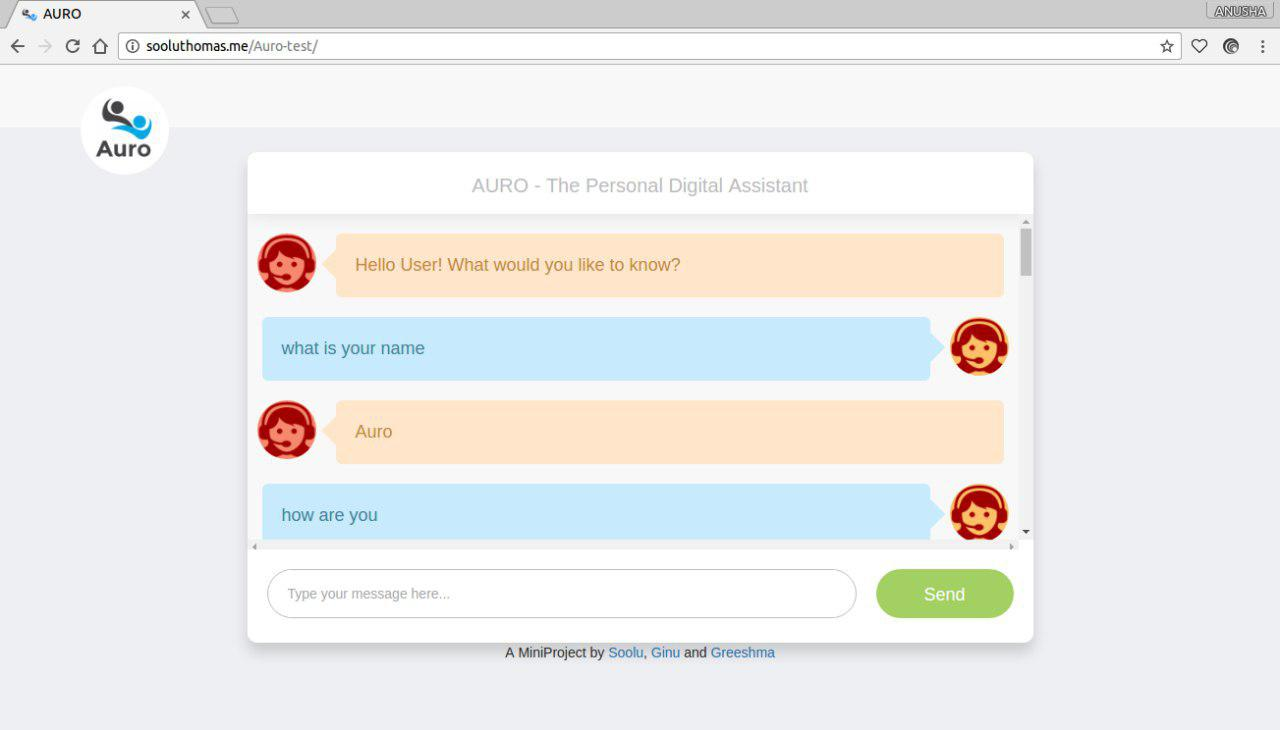
\includegraphics[width=1.1\textwidth]{3.jpg} 
  \label{fig:3}
\end{figure}

\begin{figure}[!h]
%\hspace{.1cm}
\vspace{.05cm}
  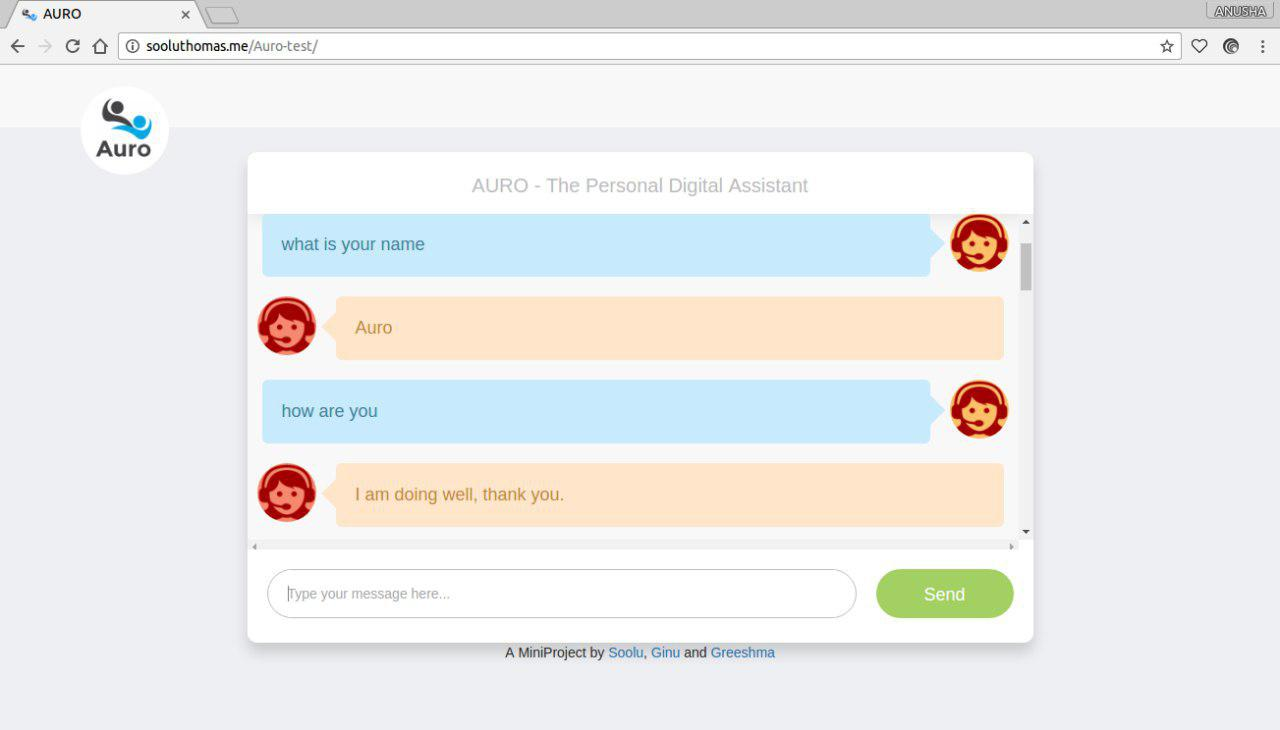
\includegraphics[width=1.1\textwidth]{2.jpg} 
  \label{fig:2}
\end{figure}

\begin{figure}[!h]
%\hspace{.1cm}
\vspace{.5cm}
  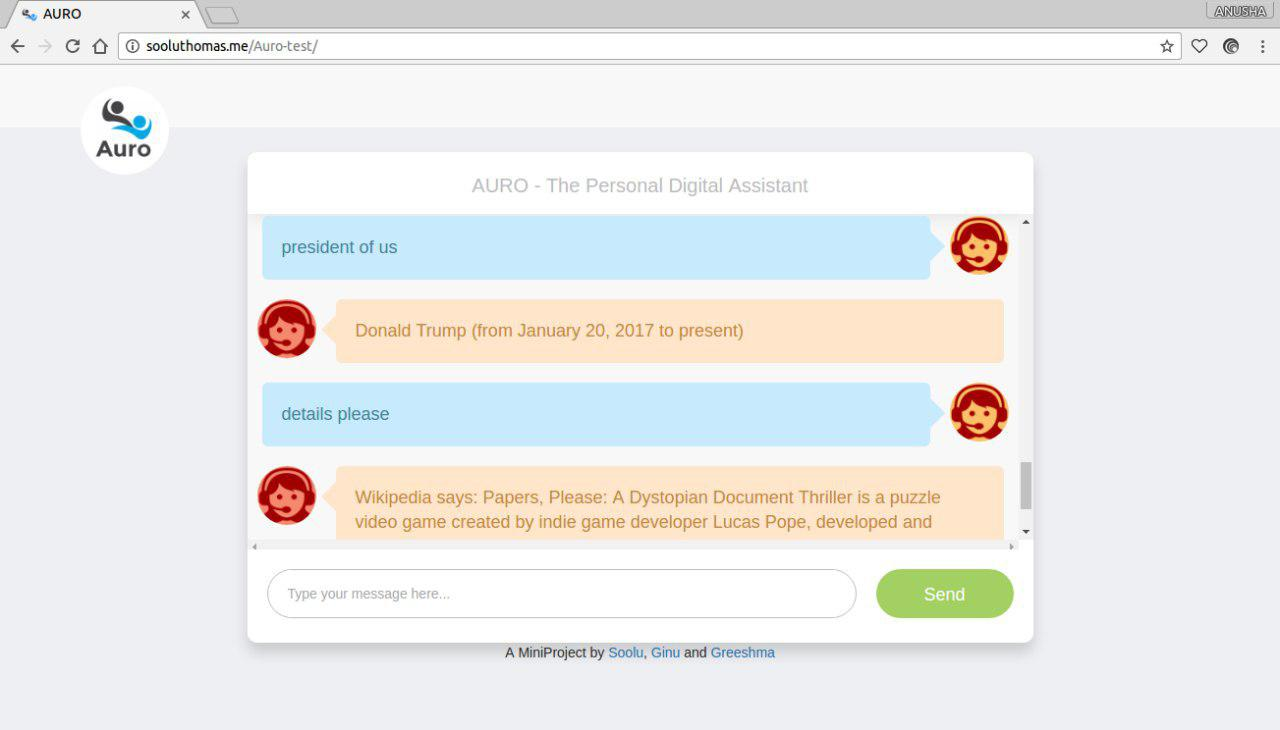
\includegraphics[width=1.1\textwidth]{4.jpg} 
  \label{fig:4}
\end{figure}

\begin{figure}[!h]
\vspace{2cm}
  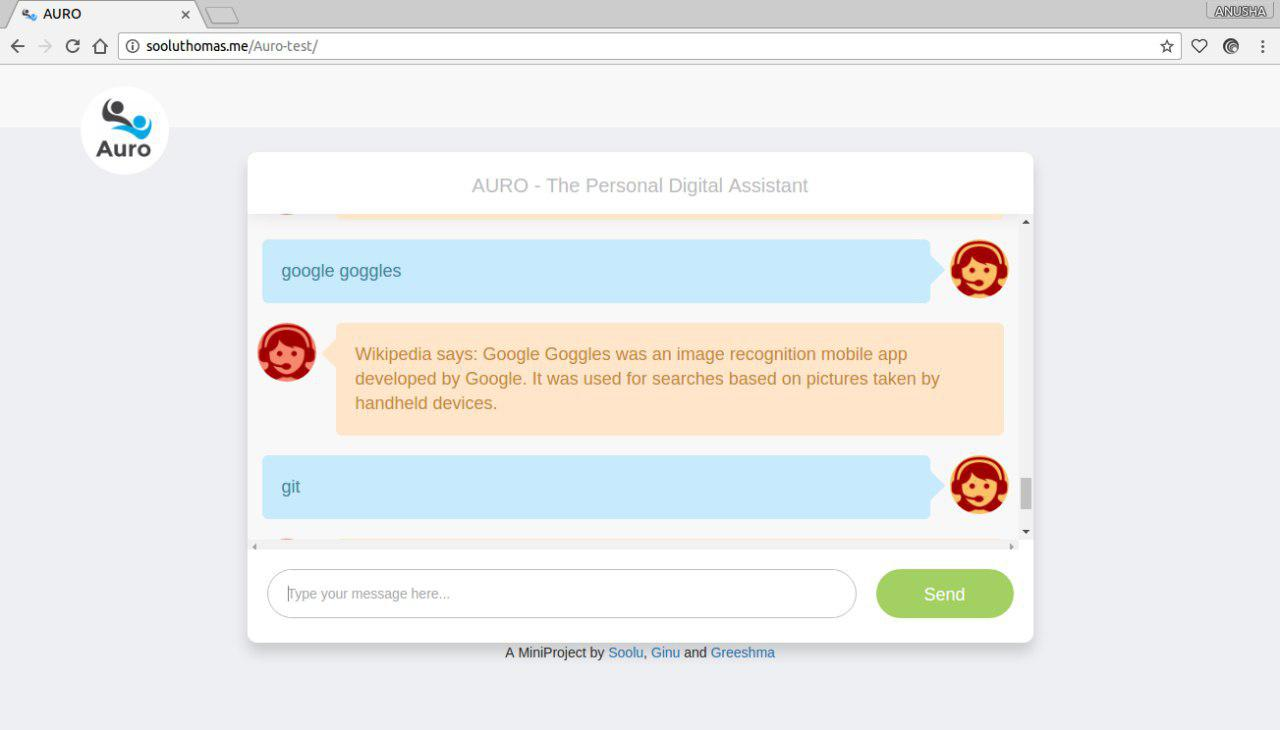
\includegraphics[width=1.1\textwidth]{1.jpg} 
  \label{fig:1}
\end{figure}

\begin{figure}[!h]
%\hspace{.1cm}
\vspace{.5cm}
  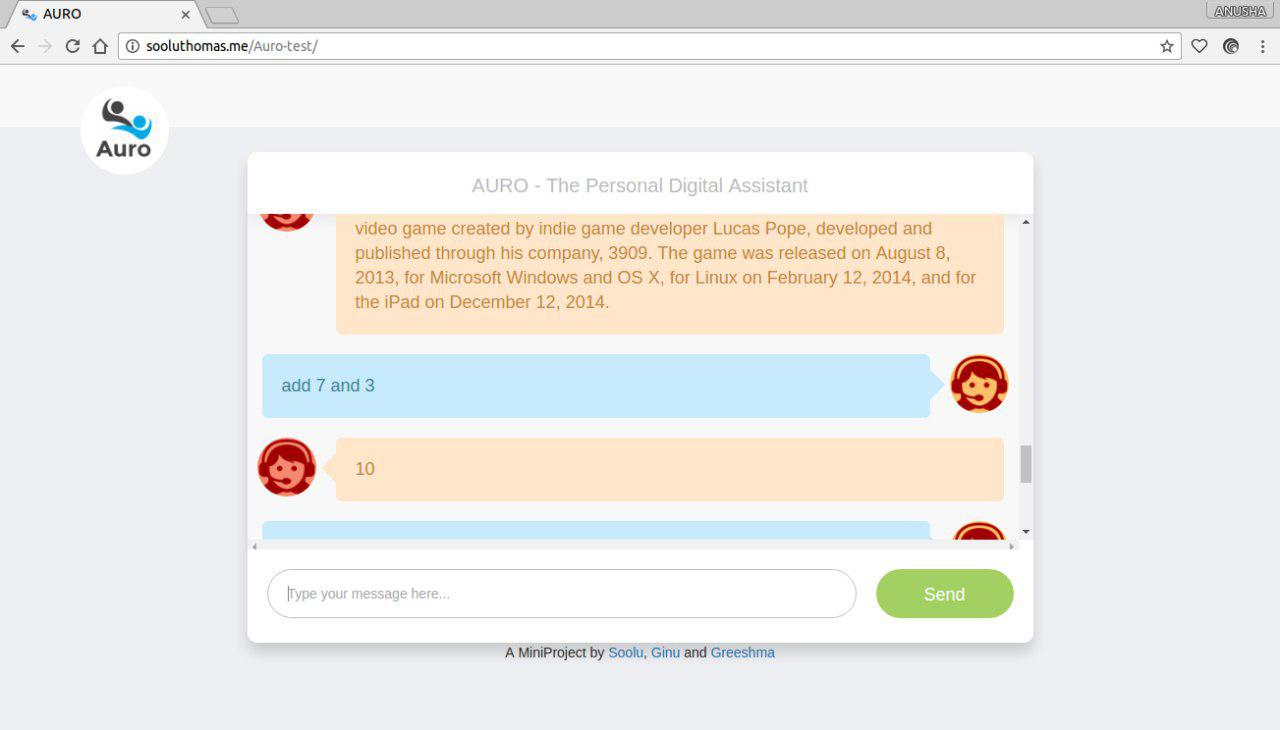
\includegraphics[width=1.1\textwidth]{5.jpg} 
  \label{fig:5}
\end{figure}

\begin{figure}[!h]
%\hspace{.1cm}
\vspace{.5cm}
  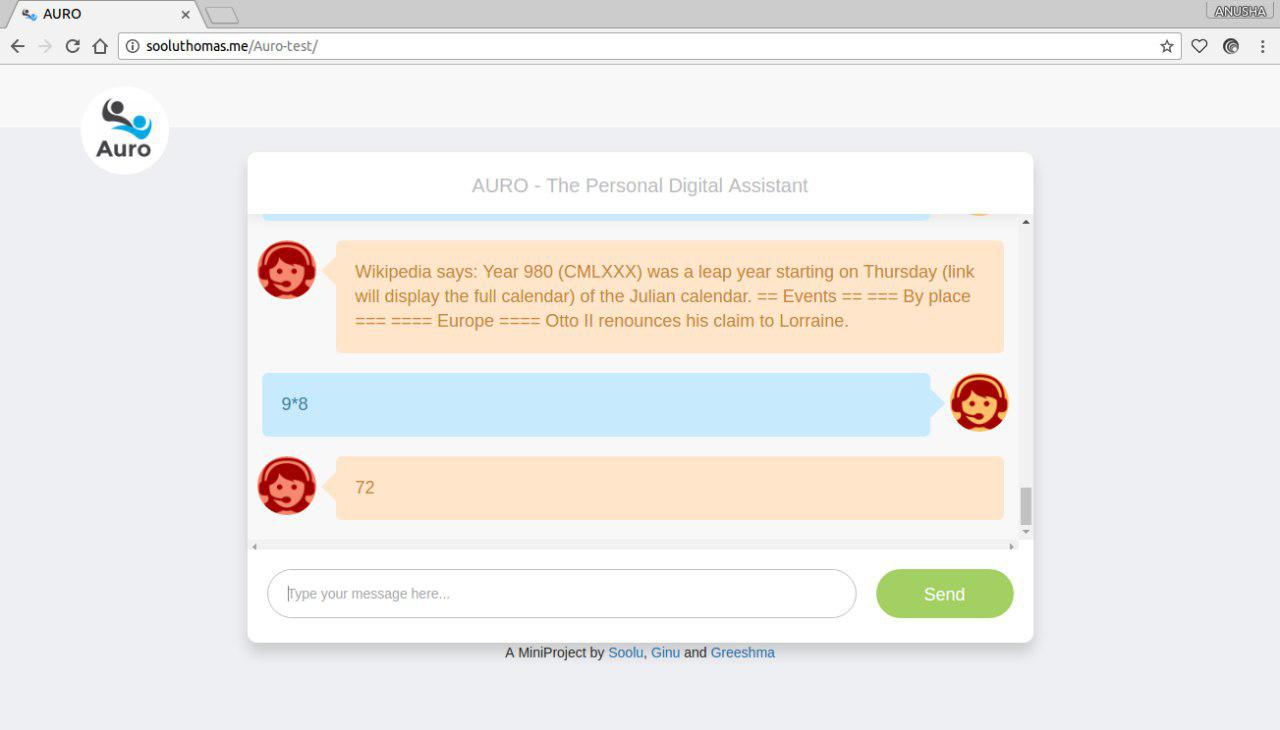
\includegraphics[width=1.1\textwidth]{6.jpg} 
  \label{fig:6}
\end{figure}

\renewcommand\bibname{References}
\begin{thebibliography}{9}
\bibitem{ieee} 
[IEEE Standard 181-1998]: The standard followed by the current SRS
 
\bibitem{pressman} 
Roger.S.Pressman, Software Engineering: A Practitioner’s Approach, McGraw Hill International edition, Seventh edition.
 
\bibitem{morgan} 
Synthesis Lectures on Human Language Technologies, Morgan \& Claypool, 2015

\bibitem{gobinda}
Natural Language Processing Gobinda G. Chowdhury Dept. of Computer and Information Sciences University of Strathclyde, Glasgow G1 1XH, UK

\bibitem{python}
Core Python Programming Wesley J. Chun Publisher: Prentice Hall PTR First Edition December 14, 2000

\bibitem{web1}
Website Reference for Natural Language Processing in Python.
Link: \textit{http://pythonprogramming.net}

\bibitem{heaton}
Artificial Intelligence for Humans, Volume 3: Deep Learning and Neural Networks, Jeff Heaton,Copyright    2015 by Heaton Research, Inc.

\bibitem{nltk}
Natural Language ToolKit for NLP in Python
Link: \textit{http://www.nltk.org}

\end{thebibliography}



\end{document}